%!TEX root = ../../../main.tex

\section[VCSELs]{Coupling \Nds to \Vcsels} \label{sec::coupling_vcsel}

For metrology, the photon flux rate has to be high enough to be measured by a low optical flux detector \cite{Vaigu2017}.

	\subsection{Pick-And-Place Process to \Vcsel}

	\begin{figure}[tp]
		\begin{subfigure}[t]{ 0.49\linewidth}
			\centering
			\testbox{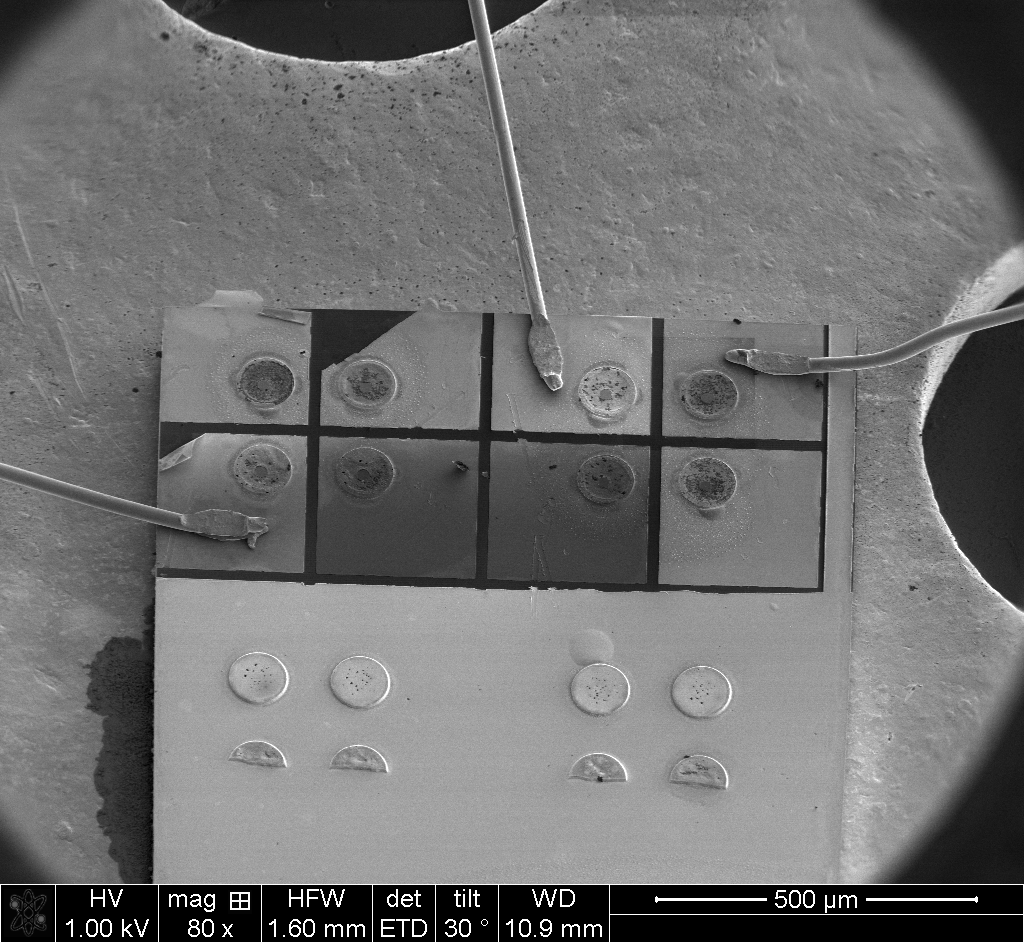
\includegraphics[trim = 0 0 0 0,  clip= true, width = \textwidth]{./pics/M05-13_PP_194_140926_13.png}}
			\caption{}
			\label{subfig::vcsel_sem_big_overview}
		\end{subfigure}
		\hfill
		\begin{subfigure}[t]{ 0.49\linewidth}
			\centering
			\testbox{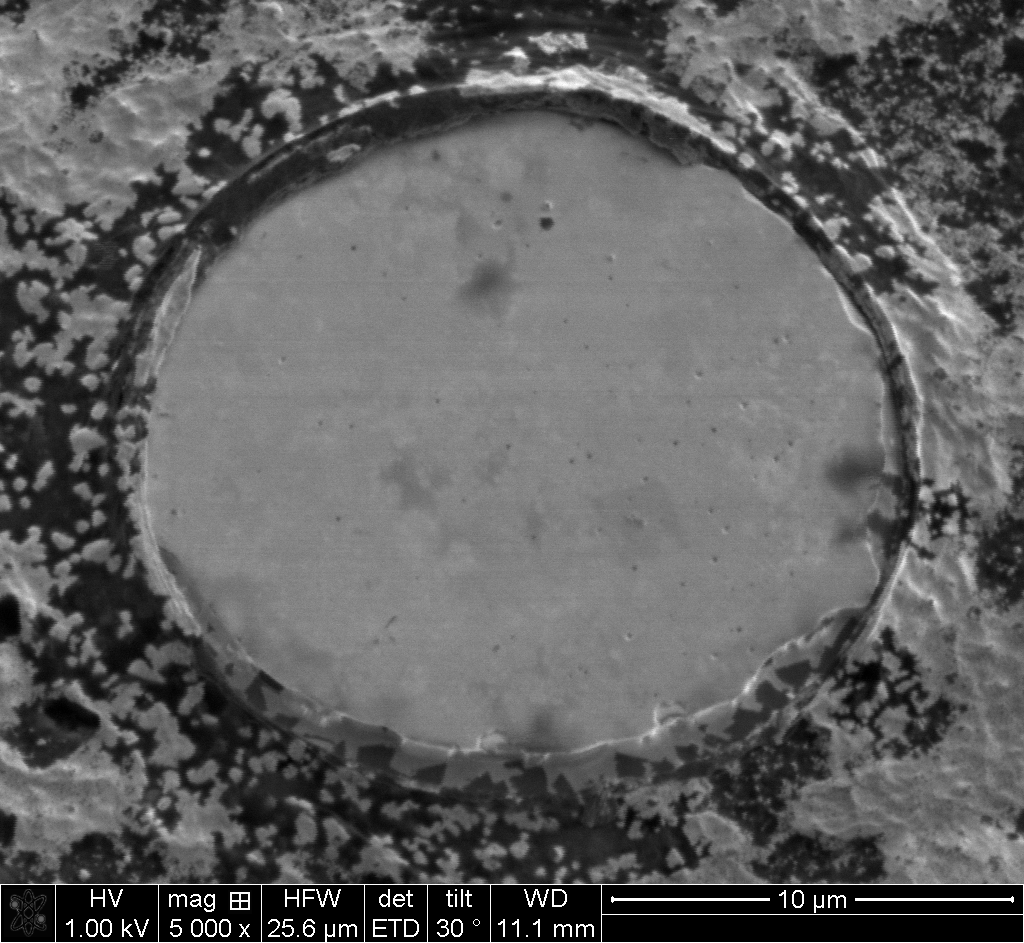
\includegraphics[trim = 0 0 0 0,  clip= true, width = \textwidth]{./pics/M05-13_PP_194_140926_14.png}}
			\caption{}
			\label{subfig::vcsel_sem_detail}
		\end{subfigure}
		\caption{<caption>}
	\end{figure}

	\subsection{Spectroscopic Measurements of \Nd in \Vcsel}

	\begin{figure}[tp]
		\begin{subfigure}[t]{ 0.49\linewidth}
			\centering
			\testbox{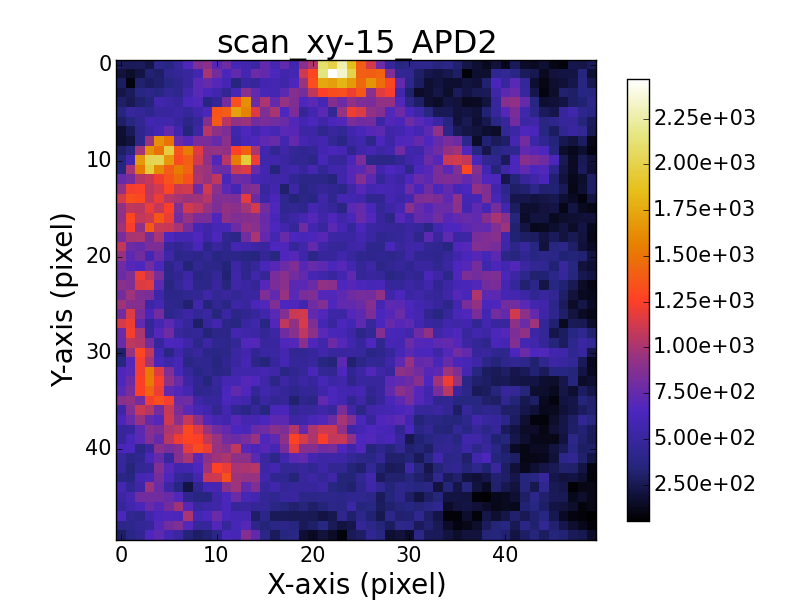
\includegraphics[trim = 0 0 0 0,  clip= true, width = \textwidth]{./pics/scan_xy-15_APD2.png}}
			\caption{confocal laser excitation with diamond}
			\label{subfig::vcsel_confocal_laser_excitation_with_diamond}
		\end{subfigure}
		\hfill
		\begin{subfigure}[t]{ 0.49\linewidth}
			\centering
			\testbox{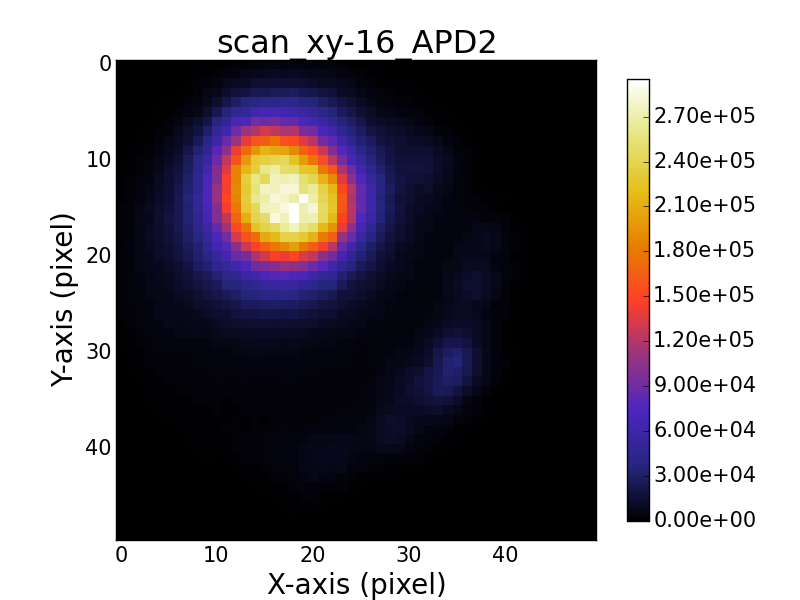
\includegraphics[trim = 0 0 0 0,  clip= true, width = \textwidth]{./pics/scan_xy-16_APD2.png}}
			\caption{vcsel excitation with diamond}
			\label{subfig::vcsel_excitation_with_diamond}
		\end{subfigure}
		\caption{}
	\end{figure}

	\begin{figure}[tp]
		\begin{subfigure}[t]{ 0.49\linewidth}
			\centering
			\testbox{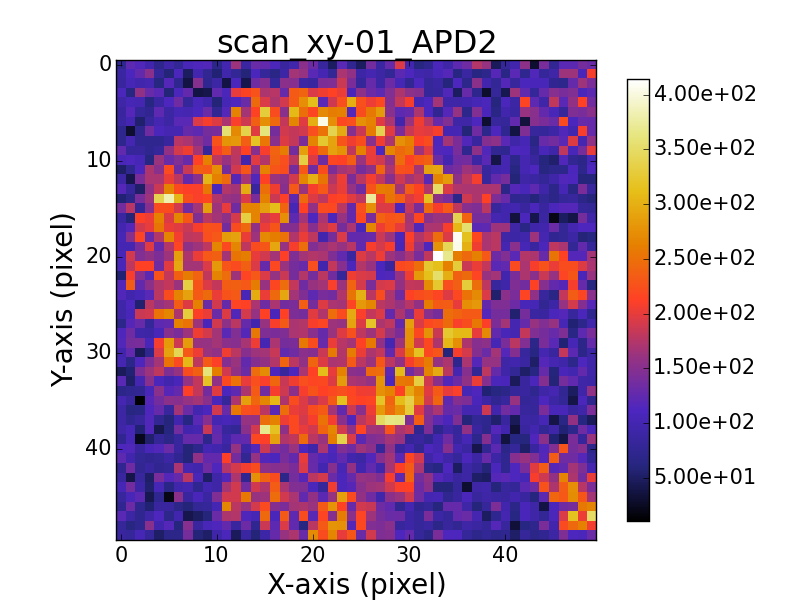
\includegraphics[trim = 0 0 0 0,  clip= true, width = \textwidth]{./pics/scan_xy-01_APD2.png}}
			\caption{confocal laser excitation without diamond}
			\label{subfig::confocal_laser_excitation_without_diamond}
		\end{subfigure}
		\hfill
		\begin{subfigure}[t]{ 0.49\linewidth}
			\centering
			\testbox{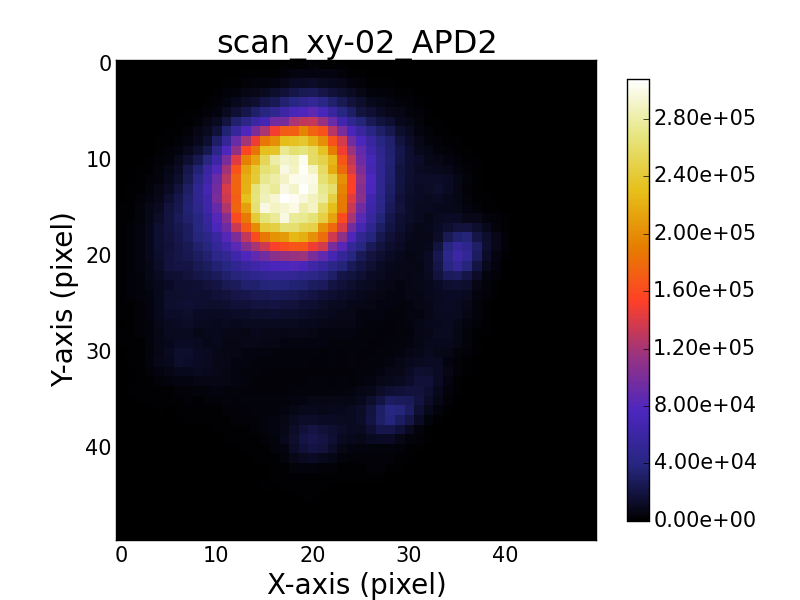
\includegraphics[trim = 0 0 0 0,  clip= true, width = \textwidth]{./pics/scan_xy-02_APD2.png}}
			\caption{vcsel excitation without diamond}
			\label{subfig::vcsel_excitation_without_diamond}
		\end{subfigure}
		\caption{<caption>}
	\end{figure}

	\begin{figure}[tp]
		\begin{subfigure}[t]{ 0.49\linewidth}
			\centering
			\testbox{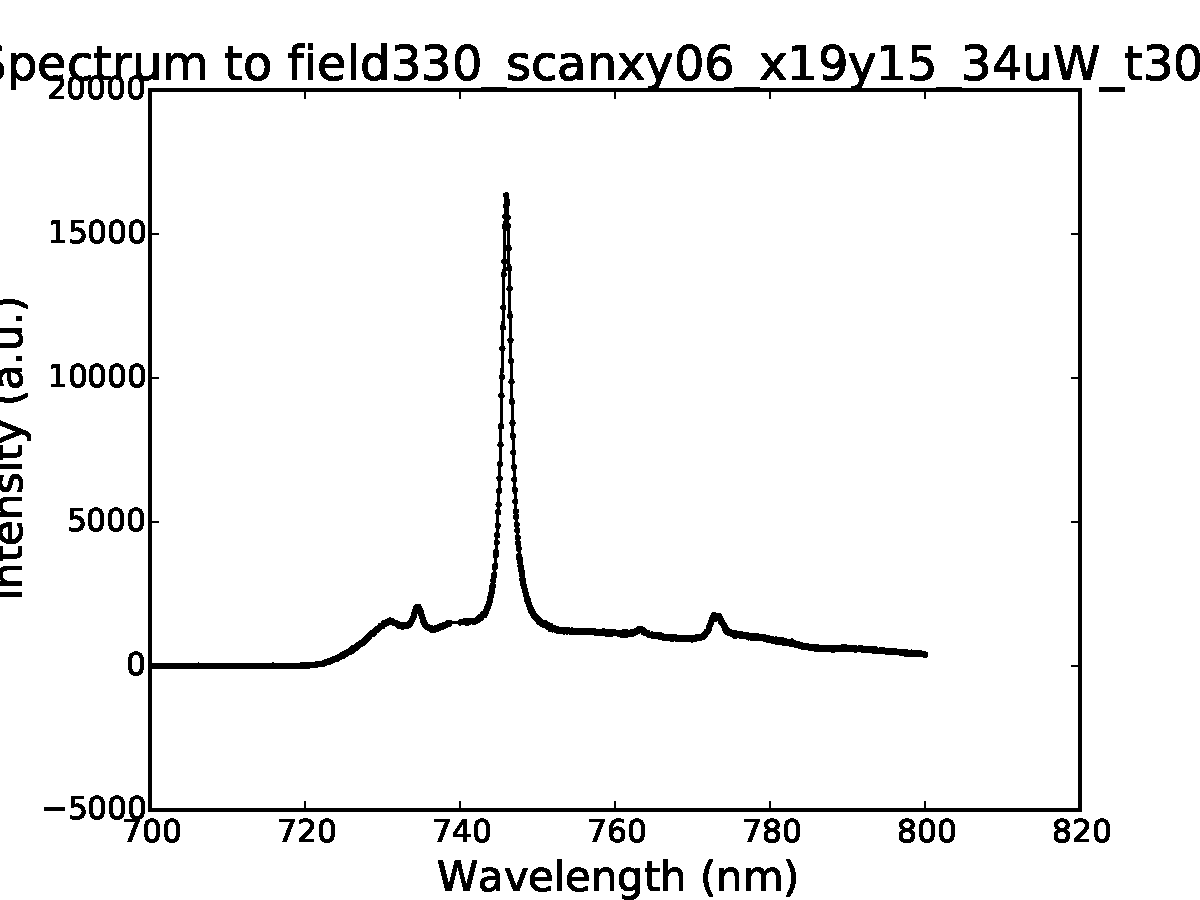
\includegraphics[trim = 0 0 0 0,  clip= true, width = \textwidth]{./pics/field330_scanxy06_x19y15_34uW_t30_2.pdf}}
			\caption{<caption>}
			\label{subfig::spectrum_diamond_for_vcsel_before_pp}
		\end{subfigure}
		\hfill
		\begin{subfigure}[t]{ 0.49\linewidth}
			\centering
			\testbox{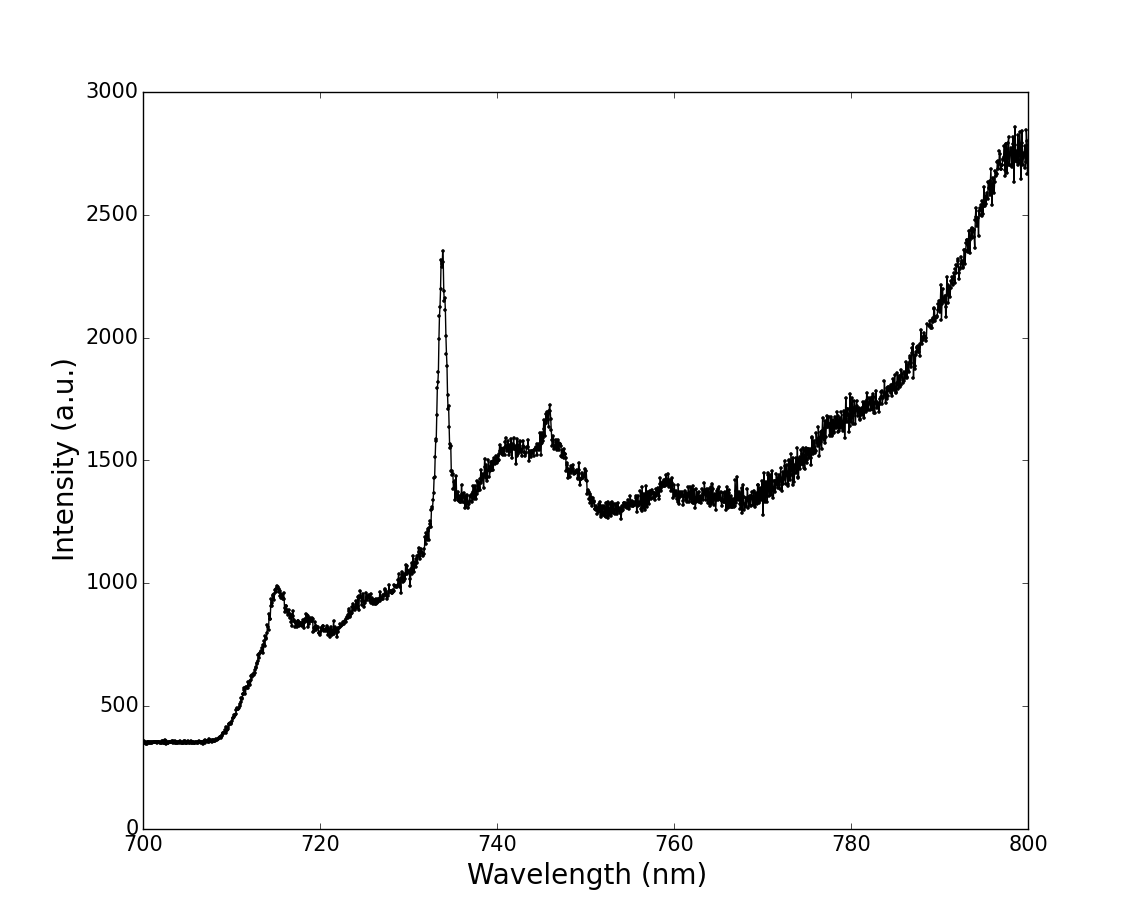
\includegraphics[trim = 0 0 0 0,  clip= true, width = \textwidth]{./pics/spe_scan_xy-25_300uW_t60_700-800nm.png}}
			\caption{<caption>}
			\label{subfig::spectrum_vcsel_confocal_excitation_with_diamond}
		\end{subfigure}
		\caption{<caption>}
		\label{fig::<fig>}
	\end{figure}

	\begin{figure}[tp]
		\begin{subfigure}[t]{ 0.49\linewidth}
			\centering
			\testbox{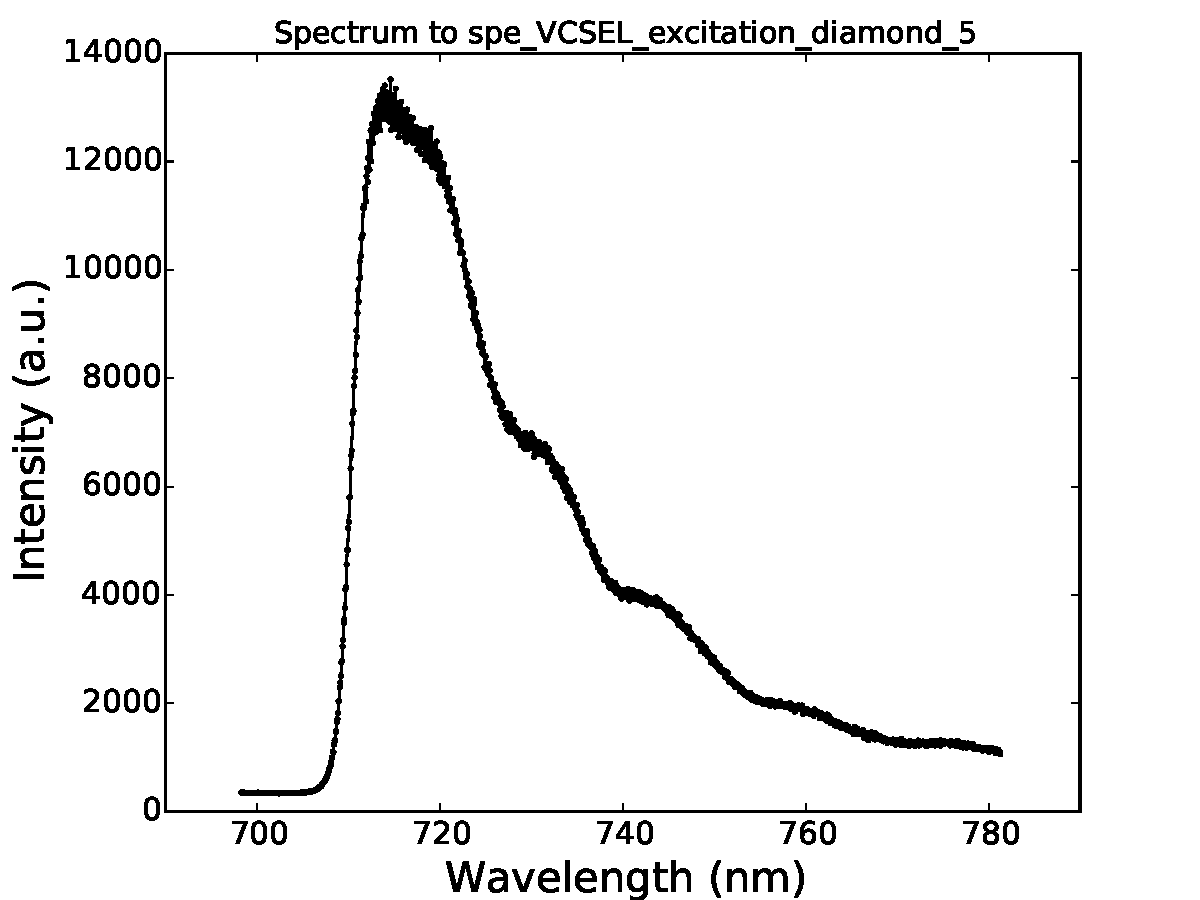
\includegraphics[trim = 0 0 0 0,  clip= true, width = \textwidth]{./pics/spe_VCSEL_excitation_diamond_5.pdf}}
			\caption{spectrum vcsel excitation with diamond}
			\label{subfig::spectrum_vcsel_excitation_with_diamond}
		\end{subfigure}
		\hfill
		\begin{subfigure}[t]{ 0.49\linewidth}
			\centering
			\testbox{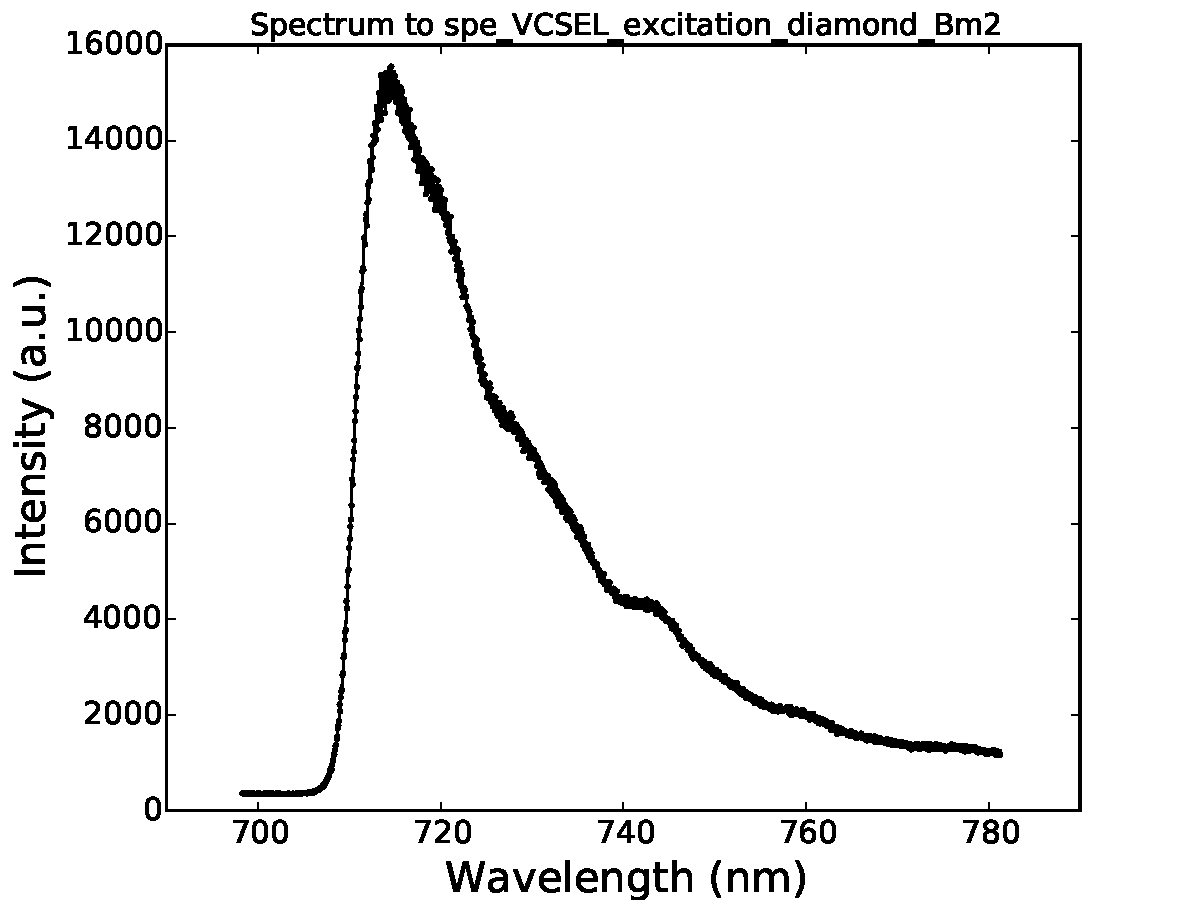
\includegraphics[trim = 0 0 0 0,  clip= true, width = \textwidth]{./pics/spe_VCSEL_excitation_diamond_Bm2.pdf}}
			\caption{spectrum vcsel excitation without diamond}
			\label{subfig::spectrum_vcsel_excitation_without_diamond}
		\end{subfigure}
		\caption{<caption>}
		\label{fig::<fig>}
	\end{figure}